\chapter{Introduction}

\section{Motivation}
The medical discipline of pathology is in a digital transformation. Instead of looking at tissue samples through the means of traditional light microscopy, it is now possible to digitize those samples. This digitalization is done with the help of a so called slide scanner. The result of such an operation is a \emph{whole slide image} (WSI)\nmc{WSI}{Whole Slide Image}\cite{Cornish13}. The digital nature of WSIs opens the door to the realm of image processesing and analysis which yields certain benefits, such as the use of image segmentation and registration methods to support the pathologist in his/her work.

A very promising approach to image analysis is the use of deep learning, also known as \emph{neural networks} (NN)\nmc{NN}{Neural Network}. These are a group of computational models inspired by our current understanding of biological NN. The construct of many interconnected neurons is considered a NN (both in the biological and artificial context). Each single one of those neurons has input values and an output value. Once the input reaches a certain trigger point, the cell in the neuron sends a signal as output. The connections between the neurons are weighted and can dampen or strengthen a signal. Because of this, old pathways can be blocked and new ones created. In other words, a NN is capable of "learning"\cite{Kriesel07}. This is a huge advantage compared to other software models. While certain problems are "easier" to solve in a sequential, algorithmic fashion (say an equation or the towers of hanoi), certain problems (e.g. image segmentation or object recognition) are very complex, so that new approaches are needed, while other problems can not be solved algorithmically at all. With the use of adequate training samples, a NN can learn to solve a problem, much like a human.

\begin{figure}[ht]
	\begin{center}
		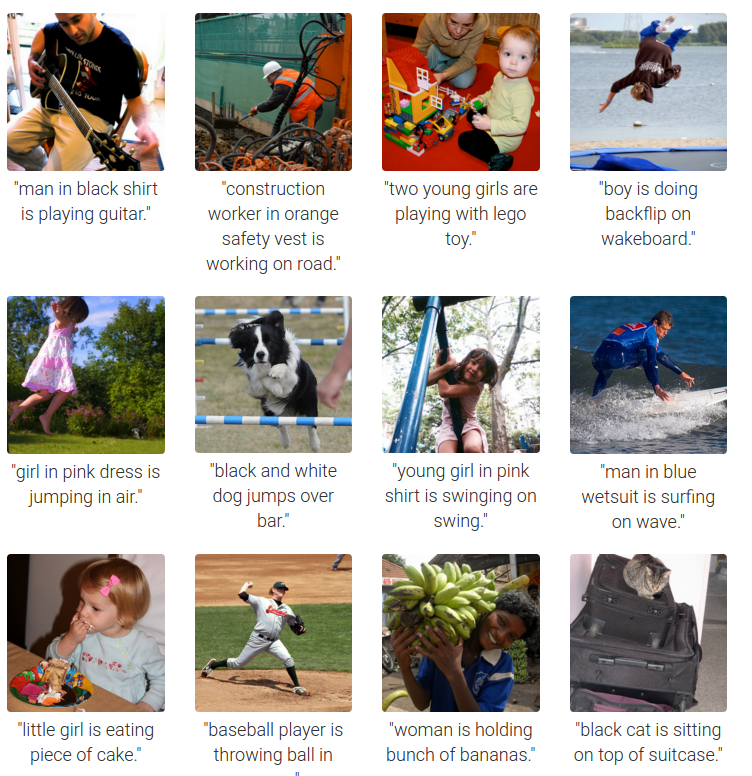
\includegraphics[scale=0.3]{img/deepVisual.png}
		\caption{Example results of the in \cite{Karpathy15} introduced model (source: \url{http://cs.stanford.edu/people/karpathy/deepimagesent/})}
		\label{fig1_karpathy}
	\end{center}
\end{figure}

In the recent past the use of NN enabled major breakthroughs, especially in the area of image classification and object recognition. Karpathy and Fei-Fei, for example, created a NN that is capable of describing an image or a scene using natural language text blocks \cite{Karpathy15} (see fig. \ref{fig1_karpathy} for a selection of examples).

There is enormous potential in the use of NN in the digital pathology as well, but to transfer these models and technologies, certain obstacles must be overcome. One of those is the need for proper training samples. While generally there are large amounts of WSIs (e.g. publicly available at the Cancer Genome Atlas\footnote{\url{https://gdc-portal.nci.nih.gov/}}), most of them will not be usable as a training sample without further preparation.

A possible way to prepare them is by using image annotation: tagging regions of interest (ROI)\nmc{ROI}{Region of Interest} on an image and assigning labels or keywords as metadata to those ROIs. These can be added to the WSIs, stored and later used for training. The result of such an approach could be similar to the one of Karpathy and Fei-Fei\cite{Karpathy15}, but with a medical context instead of daily situations.


\section{Research Objective}
\label{sec1_researchObjective}
The goal of this thesis is the conceptualization and implementation of tools to enable deep learning and pathology experts to cooperate in annotating WSIs to create a ground truth for the later use in NNs. In order to do so, it must be possible to open a given WSI with a viewer, add annotations to it and persist those annotations. Additionally, persisted annotations must be extracted from the WSI to be used as ground truth.

%Since there is no WSI file format standard, vendors developed their own proprietary solutions\cite{Cornish13}. This either leads to


%\begin{enumerate}[(i)]
%	\item locking-in on a specific vendor or
%	\item separate handling of each proprietary format
%\end{enumerate}

%(i) would render the whole process vendor specific, limiting its use drastically. (ii) would not render the process chain vendor specific but demand additional work and maintenance, due to the need of implementing multiple drivers for different formats. To counteract this, open file formats, such as the Deep Zoom Image format, have been specified\cite{Cornish13}. Additionally, converters and wrappers exist, that help to void the stated issues (i) and (ii). 

This thesis has three objectives:
\begin{enumerate}[(1)]
	\item There is no standard for WSI files, therefore vendors developed their own proprietary solutions\cite{Cornish13}. This either leads to a vendor lock-in or separate handling of each proprietary format. To avoid both cases, a conversion tool that turns proprietary WSI formats into an open format must be introduced.
	\item The deployment of a WSI viewer tool. This WSI viewer must be capable of adding annotations to a WSI and persisting them. As stated earlier, the tool is intended to be used by deep learning and pathology experts. An intuitive and easy-to-understand graphical user interface (GUI)\nmc{GUI}{Graphical User Interface} is necessary to avoid long learning periods and create willingness to actually use the tool.
	\item The implementation of a tool that is capable of turning persisted annotations into a format usable as ground truth.
\end{enumerate}

It is explicitly stated, that the intention of this thesis is to introduce tools that are used by deep learning and pathology experts to create a ground truth for NN. The intention is \textbf{not} to create a tool for analyzing and diagnosing WSIs, that is capable of competing with existing industry solutions.


\section{About this thesis}
This thesis contains 6 chapters.

\emph{Chapter 1 - Introduction} and \emph{2 - Background} address the scope, background and vocabulary of this thesis.

The chapters 3 to 5 address the components described in the last section: \emph{chapter 3 - Conversion Service} will describe a tool for image conversion, \emph{chapter 4 - Annotation Service} will describe a tool for image annotation and \emph{chapter 5 - Tessellation Service} will describe an extraction tool, to prepare the annotations made with the Annotation Service for the use in a NN.

Finally, \emph{Chapter 6 - Conclusion} will discuss and conclude the findings of the aforementioned chapters.